% begin module limit-at-infinity-ex2
\begin{frame}
\begin{example}[Example 4, p. 129]
\begin{columns}[c]
\column{.5\textwidth}
\ \only<handout:0| -5>{%
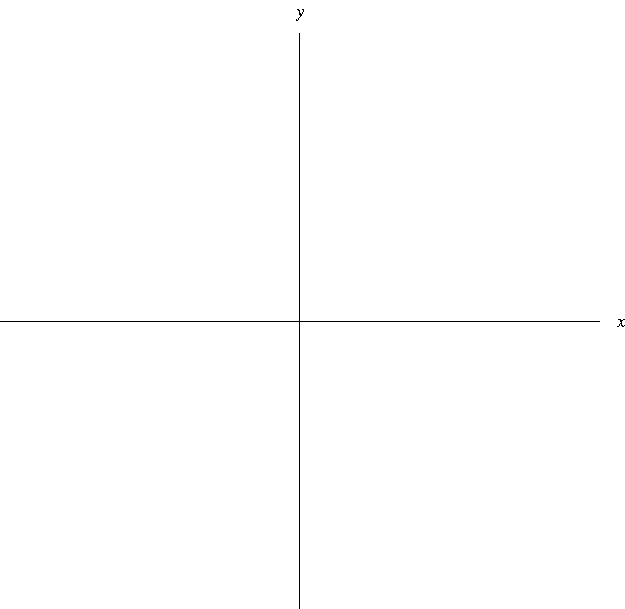
\includegraphics[width=5cm]{curve-sketching/pictures/04-04-ex2a.pdf}%
}%
\only<6->{%
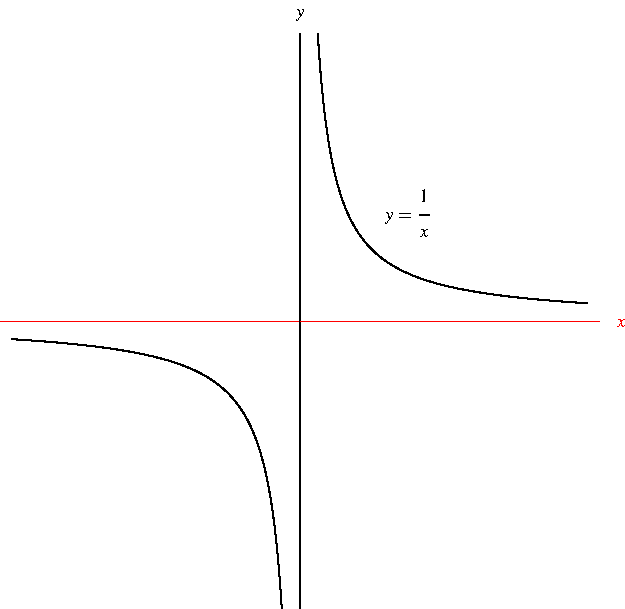
\includegraphics[width=5cm]{curve-sketching/pictures/04-04-ex2b.pdf}%
}%
\uncover<2->{%
\abovedisplayskip=0pt
\belowdisplayskip=0pt
\[
\frac{1}{100}  =  0.01, \qquad  \frac{1}{10,000}  =  0.0001
\]
\abovedisplayskip=0pt
\belowdisplayskip=0pt
\[
\frac{1}{1,000,000}  =  0.000001
\]
}%
\column{.5\textwidth}
Find $\lim_{x\to\infty} \frac{1}{x}$ and $\lim_{x\to -\infty} \frac{1}{x}$.
\begin{itemize}
\item<2->  When $x$ is large, $\frac{1}{x}$ is small.
\item<3->  By taking $x$ large enough, we can make $\frac{1}{x}$ as small as we like.
\item<4->  Therefore $\lim_{x\to \infty} \frac{1}{x} = 0$.
\item<5->  Similarly, $\lim_{x\to -\infty}\frac{1}{x} = 0$.
\item<6->  $y = 0$ (the $x$-axis) is a horizontal asymptote for the curve $y = \frac{1}{x}$.
\end{itemize}
\end{columns}
\end{example}
\end{frame}
% end module limit-at-infinity-ex2
